\documentclass[12pt, a4paper]{article}

\usepackage{setspace, graphicx, lineno, caption, color, float}
\usepackage{amsmath}
\usepackage{amsfonts}
\usepackage{amssymb}
\usepackage{amsthm}
\usepackage{amstext} %to enter text in mathematical formulae
\usepackage{algpseudocode}%psuedo code and 
\usepackage{algorithm}%puts the psuedo code in a float box
\usepackage[retainorgcmds]{IEEEtrantools}
\usepackage{natbib}
%\usepackage{url, hyperref, makeidx, fancyhdr, booktabs, palatino}
%\usepackage{euscript} %EuScript, command: \EuScript, for letters in Euler script
%\usepackage{paralist} %listing (i), (ii), etc.
\usepackage{rotating} %rotating text
\usepackage{multirow} %connecting columns in tables
\usepackage{multicol}
\usepackage{longtable}
\usepackage{array}
%image stuff
%\usepackage{epstopdf}
%\usepackage{cancel}
%\usepackage[ngerman, english]{babel} %for different languages in one document
%\usepackage[utf8]{inputenc}
%\hypersetup{colorlinks=true, linkcolor=blue}
%page set up

\usepackage[left=2.5cm,top=2.5cm,right=2.5cm, bottom=2.5cm,nohead]{geometry}
\doublespacing
%paragraph formatting
\setlength{\parskip}{12pt}
\setlength{\parindent}{0cm}

\newcolumntype{x}[1]{>{\centering\let\newline\\\arraybackslash\hspace{0pt}}p{#1}}

\begin{document}
%Make a title page
\title{The paradox of metabolic and target site resistance: How can there be both in the same population}
\author{Shaun R. Coutts$^\ddag$, Rob Freckleton$^\dag$, Helen Hick$^\dag$, Dylan Childs$^\dag$, }
\maketitle
\section{Introduction}
Often control of weed populations assumes the population will not adapt or respond to control actions, and the efficacy of any control remains constant. In reality any effective control method will impose selective pressure on a population, making that method less effective over time. Herbicide is a common tool for weed control, and as a result there is wide spread herbicide resistance. This resistance is conferred through two main mechanisms, metabolic resistance and target site resistance. Metabolic resistance involves many different stress tolerance pathways, and is thus controlled by many different genes, each having a relativity small effect. This type of trait is known as a quantitative trait and is modelled using the tools of population genetics. Target site resistance occurs when a mutation (often in a single gene) alters the binding site of the herbicide or protein affected by the herbicide. We model target site herbicide resistance as a single loci gene with two alleles, resistant and susceptible. Both target site resistance and herbicide resistance are wide spread black grass (ref) along with many other plant and insect pest species (ref). We look at the conditions under which both metabolic and target site resistance can arise in the same population relatively quickly (historically both types of resistance have developed quickly in multiple populations of different species).  

We develop a spatially explicit, density dependent population model for the economically important weed, black grass (\textit{Alopecurus myosuroides} Huds.). Specifically we test if metabolic resistance can block target site resistance from taking hold in a population by reducing the selective pressure between target site resistant and non-resistant individuals, and if so under which range of costs for metabolic resistance. We also look at the effect of gene dispersal on the simultaneous development of both target site and metabolic resistance in the same population. Clumping of genotypes (due to dispersal limitation in seeds and pollen) could allow target site resistance to take hold more quickly, since individuals with rare genotypes (like initial target site resistant mutants) will be more likely to cross with other rare mutants if closely related individuals exist spatially close to each other (i.e. sibling-sibling crosses and parent-child crosses). However, once target site resistance is established dispersal limitation will restrict its spread through the population. 

\subsection{System model}
We model the black grass population on a 1D landscape using a yearly time step, starting at the beginning of the growing season before any seeds have emerged. Survival under herbicide is conferred by two type of resistance traits, quantitative and target site. Quantitative traits are controlled by multiple genes, each having a small effect on and individuals resistance to herbicide. This leads to normally distributed resistance scores ($g$ in Eq. \ref{eq:fecund}) within the population. This quantitative resistance trait is always present in the population. That is all individuals have some value for $g$, but that value may be very small, and so phenotypically individuals are susceptible. Target site resistance is conferred by a single gene that affects the herbicides binding site. This can give almost perfect resistance to a herbicide, with little to no demographic cost. We assume target site resistance is controlled by a single loci, with inheritance following simple two allele gene and random mating. We denote the resistant allele $R$ and the susceptible allele $r$. 

These two mechanisms of resistance will interact, target site resistant individuals can survive herbicide application without the demographic costs associated with metabolic resistance. This means that target site resistant individuals can have lower levels of metabolic resistance. These low metabolic resistance genes can then spread to the rest of the population, once they develop sufficiently high numbers in the target site resistant portion of the population. All seeds in the seed bank  at location $x$, time $t$, with genotype $G$ are distributed over metabolic resistance score $g$, we denote the distribution  
\begin{equation}\label{eq:seedbank_simp}
	b(g, G, x, t + 1) = b(g, G, x, t)(1 - \phi_e)\phi_b + f(g, G, h, x, t) 
\end{equation}
Each genotype can contribute both target site resistance alleles and metabolic resistance genes to the other genotypes at all other locations. The first term is the distribution of surviving seeds in the seed bank of genotype $G$ at location $x$, and the second term is the distribution of new seeds of genotype $G$ added to the population at location $x$. There are two important points to make, the first is that $b(g, G, x, t)$ and $f(g, G, h, x, t)$ are distributions over metabolic resistance score $g$. To get the total number of seeds for genotype $G$ the distribution has to be integrated over $g$, i.e. $\int b(g, G, x, t) \text{d}g$, and the total number of seeds is $\sum_{\forall G} \int b(g, G, x, t) \text{d}g$. The second point is that the even though these distributions are on the same axis ($g$), they can be different for each genotype, i.e. $b(g, RR, x, t) \neq b(g, Rr, x, t) \neq b(g, rr, x, t)$. In fact we expect the mean each genotypes' distribution to be different. 

With both metabolic resistance (quantitative trait) and target site resistance (single loci trait) operating the distribution of new seeds over metabolic resistance score $g$ arriving at location $x'$ is      
\begin{align}
\label{eq:fecund}
\begin{split}
	f(g, G, &h, x', t) = \displaystyle \sum_{\forall G_m}\sum_{\forall G_p} Q(G, G_m, G_p) \int_{x_m}\int_{x_p}\int_{g_m}\int_{g_p} \text{N}(0.5 g_m + 0.5 g_p, \sigma_f)\cdot\\
	&n(g_m, G_m, x_m, t)s(g_m, G_m, x_m, h_x)\psi(g_m, x_m)d_m(x_m, x')\cdot \\
	&\frac{n(g_p, G_p, x_p, t)s(g_p, G_p, x_p, h_x)d_p(x_p, x_m)}{\sum_{\forall G}\int_{x}\int_{g_p} n(g_p, G, x, t)s(g_p, G, x, h_x)d_p(x, x_m)\text{d}g_p\text{d}x} \text{d}g_m \text{d}g_p\text{d}x_m\text{d}x_p
\end{split}
\end{align}           
and is the result of three mixing kernels. The first mixes genes within and between target site resistance genotypes. This mixing kernel comprises a double summation over maternal and paternal target site genotypes ($G_m$ and $G_p \in \{\{R, R\}, \{R, r\}, \{r, r\} \}$) and the mixing function $Q(G, G_m, G_p)$. The second mixing kernel (double integration) gives the expected distribution of seeds over metabolic resistance score $g$, given the maternal and paternal parent distributions for each combination of target site resistance genotypes. Thus Eq. \ref{eq:TSR_mixing_kern} mixes the quantitative genetic trait with and between each parental genotype. The target site mixing function is
\begin{subequations}
\begin{equation}\label{eq:TSR_mixing_kern}
	Q(G, G_m, G_p) = \frac{\sum_{\forall k \in G_m \times G_p} q(G, k)}{card\left( G_m \times G_p \right)}
\end{equation}      
\begin{equation}\label{eq:allel_count}
	q(G, k) = \begin{cases}
		1 &\text{if } a_1 \in k \bigwedge a_2 \in k\\
		0 &\text{otherwise} 
	\end{cases}, \text{where } G = \{a_1, a_2\}
\end{equation} 
\end{subequations}
This function uses set notation that may be unfamiliar so I will go through it carefully and give an example. $Q(G, G_m, G_p)$ is the fraction of seeds produced of target site genotype $G$ by parents of target site genotype $G_m$ and $G_p$. We assume that target site resistance is a single loci trait. Thus, each genotype can be thought of as a set of two alleles, $G = \{a_1, a_2\}$, with $a_i \in \{R, r \}$ and full set of target site resistant genotypes is $G \in \{\{R, R\}, \{R, r\}, \{r, r\} \}$. The numerator is the number of all possible combinations of $G_m\{a_i\}$ and $G_p\{a_j\}$ that result in genotype $G$. To achieve this we use a structure called a Cartesian product. The Cartesian product of sets $X$ and $Y$ ($X \times Y$) is the set of all ordered pairs $(x, y)$, with $x \in X$, $y \in Y$ and $(x, y) = (x', y')$ if and only if $x = x'$ and $y = y'$. To give a more concrete example we explicitly write out the Cartesian product when $G_m = \{R, r\}$ and $G_p = \{R, r\}$  
\begin{equation*}
	\{R, r\} \times \{R, r\} = \{(R, R), (R, r), (r, R), (r, r)\}
\end{equation*}
The task is now to find the number of these ordered pairs which contain both alleles present in the genotype of interest, $G$. To do this we use the function $q(G, k)$. Recall that $G = \{a_1, a_2\}$ and note that the variable $k$ is iterated over $G_m \times G_p$, which is the set of all possible ordered pairs of alleles in $G_m$ and $G_p$. To extend the example above if the genotype of interest is $\{R, r\}$ then 
\begin{equation*}
	\sum_{\forall k \in \{R, r\} \times \{R, r\}} q(\{R, R \}, k) = 2
\end{equation*}    
Since only two of the ordered pairs, $(R, r)$ and $(r, R)$ contain both $a_1 = R$ and $a_2 = r$. To make this a proportion of all possible combinations we divide by the cardinality of the Cartesian product, $card \left( G_m \times G_p \right)$. For example 
\begin{equation*}
	card\left( \{R, r\} \times \{R, r\} \right) = card\left( \{(R, R), (R, r), (r, R), (r, r)\} \right) = 4
\end{equation*}

Now we have the proportion of genotype $G$ seeds produced by each combination of parental genotypes $G_m$ and $G_p$, but we still need the distribution of quantitative trait $g$ for the offspring of each combination of parental genotypes $G_m$ and $G_p$, at each location $x$. We do the quantitative trait mixing with a double integration in Eq. \ref{eq:fecund} over every combination of metabolic resistance score $g$ from the maternal parent distribution, $g_m$, and paternal distribution, $g_p$. The offspring produced by every pair of $g_m$:$g_p$ values are assumed to be normally distributed over $g$ with a mean of $0.5g_m + 0.5g_p$ and a standard deviation of $\sigma_f$ ($\text{N}(\cdot)$ in Eq. \ref{eq:fecund}). The parent distribution for each target site genotype $G$ at location $x$ is $n(g, G, x, t)s(g, G, x, t)$, where 
\begin{equation}\label{eq:above_ground}
	n(g, G, x, t) = b(g, G, x, t)\phi_e\phi_b
\end{equation}
is the number of individuals of target site genotype $G$ that emerge from the seed bank and establish. Note that because $b(g, G, x, t)$ is a distribution so is $n(g, G, x, t)$. The distribution of these emerged individuals that survive, $s(g, G, x, h_x)$, is based in their target site genotype, $G$, their metabolic resistance score, $g$, their location $x$, and whether or not herbicide is applied at location $x$, $h_x \in \{0, 1\}$.   
\begin{equation}\label{eq:sur_G}
	s(g, G, x, h_x) = \begin{cases} 
		\frac{1}{1 + e^{-s_0^x}} &\text{~if~} G \in G^* \\
		\frac{(1 - \varsigma)}{1 + e^{-s_0^x}} + \frac{\varsigma}{1 + e^{-s_0^x - h_x\left(\xi - \textbf{min}(\xi, \rho g) \right)}} &\text{~otherwise~} 		
	\end{cases} 
\end{equation}
We assume that seeds which germinate but die before seed set of non-management causes are subsumed into the seed survival term, $\phi_b$. We also assume that any reduction in survival due to increased density is subsumed into the affect of density on fecundity (Eq. \ref{eq:seed_production}). There are two ways individuals can avoid being affected by herbicide; i) they can not be exposed due to emerging later in the growing season, or they may simply be missed spatially, $\varsigma$ is the proportion of individuals exposed to the herbicide, ii) target site resistant individuals are assumed to be completely protected from the effects of the herbicide. $G^*$ is the sub-set of genotypes that give target site resistance. If $G^* \in \{\{R, R\}, \{R, r\}\}$ then target site resistance is a dominant trait and if $G^* = \{R, R\}$ then target site resistance is recessive. $s_0^x$ is the survival probability (in logits) when there is no herbicide, or for individuals not affected by herbicide, at location $x$ for individuals with resistance score $g = 0$. Notice that when $h_x = 0$ the top and bottom condition of Eq. \ref{eq:sur_G} are the same. $\xi$ is the reduction in survival (in logits) caused by herbicide for individuals with a resistance score $g = 0$ and $\rho$ is the protective effect of a one unit increase in resistance score $g$. Because $\rho$ is only meaningful in relation to $\xi$, and $\xi$ is only meaningful relative to $s_0^x$, we can fix $s_0^x \in \{10, -10\}$, for suitable and unsuitable habitat respectively, and still produce the full range of possible behaviours by choosing different values for $\rho$ and $\xi$. 

The survival due to metabolic resistance (second condition in Eq. \ref{eq:sur_G}) interacts with survival due to target site resistance. Individuals with no target site resistance will have some level of metabolic herbicide resistance (although that level may be very low). When metabolic resistance is low the difference in survival between target site resistant and non-resistant individuals (and thus the selection pressure), will be large. However, for individuals with high levels of metabolic resistance the difference in survival between target site resistant and non-resistant individuals will be small. Also metabolic resistance comes with a demographic cost, which we model as a reduction in fecundity. Target site resistant individuals require no metabolic resistance to survive herbicide application, and thus can have higher fecundity, potentially helping to drive target site resistance through the population. The number of seeds produced per individual, $\psi(g)$, is a function of resistance and the density of surviving plants, with greater resistance and higher density reducing the number of seeds. 
\begin{subequations}
\begin{equation}\label{eq:seed_production}
	\psi(g, x) = \frac{\psi_\text{max}}{1 + \Psi(g) + f_d M(h_x, x, t) + f_dM(h_x, x, t) \Psi(g)}
\end{equation}  
\begin{equation}
	\Psi(g) = 1 + e^{-(f_0 - f_r|g|)}
\end{equation}
\end{subequations}
where $\psi_\text{max}$ is the maximum possible number of seeds per individual, $f_0$ controls the number of seeds produced when $g = 0$, $|g|$ is the absolute value of $g$, $f_r$ is the cost of resistance in terms of reduction in seed production, $1/f_d$ is the population level where individuals start to interfere with each other and 
\begin{equation}\label{eq:num_sur}
   M(h_x, x, t) = \sum_{\forall G} \int_g n(g, G, x, t)s(g, G, x, h_x)\text{d}g
\end{equation}
is the number of above ground individuals that survive until seed set at location $x$. Note that we implicitly assume that pollen production is not affected by either density or metabolic resistance score $g$. This may have a marginal effect in the spatial model because pollen is more dispersive than seeds. Thus, this assumption means that high metabolic resistance genes can spread more easily across the landscape.   

The third mixing kernel mixes both target site and metabolic resistance genes spatially. Spatial mixing also requires double integration over the location of the mother, $x_m$, and father, $x_p$. This double integration over spatial locations takes every pair of locations $x_m:x_p$ and generates a distribution of seeds over metabolic resistance score $g$ for every genotype $G$ at maternal location $x_m$ based on the paternal parent distribution of survivors at paternal location $x_p$. The paternal parental distribution of survivors is weighted by the distance between the maternal and paternal locations $x_m$ and $x_p$ according to the pollen dispersal kernel 
\begin{equation}\label{eq:pollen_disp}
	d_p(i, j) = \frac{c}{a^{2/c}\Gamma\left(\dfrac{2}{c} \right)\Gamma\left(1 - \dfrac{2}{c} \right)}\left( 1 + \dfrac{\delta_{i,j}^c}{a} \right)^{-1} 
\end{equation} 
This is a logistic kernel, which was found to be the one of the best fitting pollen dispersal kernels for oil seed rape \citep{Klei2006}. This is a two parameter kernel with a scale, $a$, and shape, $c$, parameter, where $\delta_{i,j}$ is the distance between locations $i$ and $j$. For each maternal location $x_m$ the amount of each pollen type (i.e. a unique value of $g$ and $G$) arriving is divided by the total amount of pollen from every target site resistance genotype, from every location for every metabolic resistance score $g$ that arrives at the maternal location $x_m$ (double integration in denominator of Eq. \ref{eq:fecund}). The probability that a seed produced at maternal location $x_m$ is dispersed to location $x'$ is 
\begin{equation}\label{eq:seed_disp}
	d_m(i, j) = l \mu_1 \omega_1 \delta_{ij}^{\omega_1 - 2}e^{-\mu_1 \delta_{ij}^{\omega_1}} + (1 - l) \mu_2 \omega_2 \delta_{ij}^{\omega_2 - 2}e^{-\mu_2\delta_{ij}^{\omega_2}}
\end{equation} 
Weibull dispersal kernel developed by \cite{Colb2001} to model seed dispersal of black grass where $\delta_{ij}$ is the distance between locations $i$ and $j$, $l$ is the proportion of seeds in the long dispersal kernel rather than the short dispersal kernel, $\mu_{1, m}$ and $\mu_{2, m}$ control scale of the dispersal kernel for the long and short parts of the kernel, $\omega_{1, m}$ and $\omega_{2, m}$ are shape parameters for the short and long dispersal kernels.    

\section{Parametrization}
Several of the population model parameters, particularly those relating to the quantitative genetic selection model, are unknown for our study system. However, we do have field observations with estimates of above ground plant densities and susceptibility to herbicide. While we cannot directly parametrize the model with this data, we can use it to constrain the parameter space to regions that produce sensible results (i.e. those that match up with the observed densities). To do this we run the system model over 50 time steps under different parameter combinations under continual herbicide application. We can then see which parameter combinations resulted in above ground populations like those we observe in the field.  

For this approach to work well we need to constrain the parameter space as much as possible \textit{a prior}. Estimates and sources for each parameter are given in Table \ref{tab:parameters}.          

\begin{longtable}[h]{x{1.5cm} x{2.1cm} x{2cm} x{1.5cm} p{3.5cm} p{3cm}} \label{tab:parameters}\\
\caption{System model parameters}\\
	\hline
	\textbf{parameter} & \textbf{units} & \textbf{range} & \textbf{estimate} & \textbf{description} & \textbf{source}\\
	\hline
	\multicolumn{6}{l}{\underline{Population model}}\\
	$\phi_b$ & prob. & 0.22 -- 0.79 & 0.45 & seed survival & \cite{Thom1997}\\
	$\phi_e$ & prob. & 0.45 -- 0.6 & 0.52 & germination probability & \cite{Colb2006}\\	
	$\psi_\text{max}$ & seeds/plant & 30 -- 300$^\blacklozenge$ & 45 & seed production of highly susceptible individuals at low densities & \cite{Doyl1986}\\
	$f_d$ & 1 / pop. & 0 -- 0.15$^\dag$ & 0.004 & reciprocal of population at which individuals interfere with each other & \cite{Doyl1986}\\ 
	$f_0$ & logits & 5 -- 10$^\dag$ & no est$^\ddag$  & fecundity in a naive population is logit($f_0$)$\psi_\text{max}$ & simulation\\
	$f_r$ & logits & $0.1f_0$ -- $2f_0 ^\dag$ & no est$^\ddag$ & reduction in fecundity due to a one unit increase in resistance. Only meaningful in relation to $f_0$ & simulation\\
	$\sigma_f$ & arbitrary & fixed & 1 & standard deviation of offspring distribution & fixed without loss of generality\\
	$s_0$ & logits & fixed & 10 & survival in a naive population is logit($s_0$) & fixed without loss of generality\\
	\multicolumn{6}{l}{\underline{Management effects}}\\
	$\varsigma$ & prop. & 0.5 -- 1$^\dag$ & 0.8$^\blacklozenge$ & proportion of above ground individuals exposed to herbicide & HGCA\\   		
	$\xi$ & logits & $2s_0$ -- $3s_0^\dag$ & no est$^\ddag$ & reduction in survival due to herbicide (only meaningful in relation to $s_0$ & simulation\\	
	$\rho$ & logits & $0.1\xi$ -- $2\xi$ & no est$^\ddag$ & protection against herbicide conferred by a one unit increase in $g$, only meaningful in relation to $\xi$ & simulation\\
	int$_{Rr}$ & proportion & 0.001 -- 0.2 & & initial frequency of resistant target site genotype. All other individuals are assumed to be of genotype rr & simulation.'\\     
	\hline
	\multicolumn{6}{l}{$\blacklozenge$ sourced from grey literature, unpublished data and expert opinion}\\
	\multicolumn{6}{l}{$\dag$ range not available from literature, simulation used to find plausible range}\\
	\multicolumn{6}{l}{$\ddag$ no estimate not available from literature, simulation used to find plausible
	 range}
\end{longtable}

We use Latin hypercube sampling to evenly sample 24,000 parameter combinations across the parameter space. We run each set of parameters for 50 time steps with constant herbicide use, starting with an initial population of three seeds, one in each of the center three locations, with an initial frequency if the target site resistant genotype Rr, set by int$_{Rr}$. For each run we record the above ground post herbicide population after 50 time steps.    

From this dataset of 24,000 parameter combinations we filter out those parameter combinations that resulted in unrealistic population dynamics. We use data from 140 fields across England to define what realistic, resistant, populations look like. These fields were visually inspected in ??? - ???, and every 20 m by 20 m grid square was assessed as being in one of four density classes; 'absent' (0 plants/20m$^2$), 'low' (1 -- 160 plants/20m$^2$), 'medium' (160 -- 450 plants/20m$^2$), 'high'(450 -- 1450 plants/20m$^2$) and very high ($>$1450 plants/20m$^2$), coded as \{0, 1, 2, 3, 4\}. The resistance status of each field to the three most common herbicide active ingredients was determined in a glass house trial. Seeds from 100 seed heads from 10 different locations in each field were taken post herbicide application (July -- August). These seeds were raised in a glass house and divided into three groups of 12 -- 19 plants (median 18) for each field. Each group had ??? of the herbicide 'Atlantis', 'Fenoxaprop' or 'Cycloxydim' applied, mortality and any damage were recorded after ??? days. We assume that after 50 years of continuous herbicide use black grass population will be resistant, thus, we only included highly resistant fields, where survival to all herbicides was $>80\%$ (???? fields). To set the lower and upper number of blackgrass plants in winter wheat per hectare, after herbicide application, we use the mean density class of the highly resistant fields with the minimum (0.94) and maximum (4) observed mean density class. We then used the observed number of plants per 20m$^2$for each density class (calculated from \citealt{Quee2011}) and a randomization process (see appendix 1) to determine that post herbicide populations should fall between 16,348 and 132,000 plants per ha. Because our model is run on a 1D landscape, while the data are given in plants/m$^2$, estimated at a 20m resolution, we assume the modelled population occurs in a 20 m x 500 m, 1 ha field. Note that this process is not intended to definitively parametrize the model, rather is acts as a sanity check on the model outcome, removing parameter combinations that result in black grass which are never observed in the field data. Only four parameters determined if a parameter set passed this sanity check, $f_d$, $\psi_\text{max}$, $f_r$ and $\phi_b$ see appendix 1 for more details.     

\subsection{Sensitivity analysis}
The sanity check resulted in 11,710 parameter combinations that produced black grass populations which fell in the acceptable range. We performed a global sensitivity analysis on this set of 11,710 'realistic' parameter sets to explore how different parameters, and their interactions, affected the behaviour of the model. We followed the approach of \cite{Cout2014} and fit Boosted Regression Trees (BRTs) to the dataset of 11,710 sanity checked parameter combinations to find relationships between the parameter values and the model behaviours of interest. We are primarily interested in three aspects of the models behaviour. We measure the speed at which target site resistance establishes in the population as the time step, $t$, at which the resistant target site allele, R, makes up 50\% of all target site alleles in the population  
\begin{equation}\label{eq:t_R50}
	t_{R50} = \text{first } t \text{ when } \frac{\left(2\int_x\int_g b(g, \text{RR}, x, t) + \int_x\int_g b(g, \text{Rr}, x, t) \right)\text{d}x\text{d}g}{2\sum_{\forall G} \int_x\int_g b(g, G, x, t)\text{d}x\text{d}g} \geq 0.5
\end{equation}.    
Secondly we measure how quickly the black grass population spread across the landscape as $\overline{C}$, the mean number of new locations with at $\geq$ one seed in the seed bank at each time step. So that slow expansion due to a full landscape does not affect the estimate of spread speed the mean is only taken over time steps where $<$90\% of locations have $\geq 1$ seed in the seed bank. Finally we measure the relative contributions of metabolic resistance and target site resistance to the survival of black grass under herbicide as the mean proportion of individuals of target site genotype rr that survived until seed production taken over 50 time steps.  
\begin{equation}\label{eq:mean_pro_rr}
	\overline{P}_{rr} = \frac{\sum_{t=1}^{t=T}\int_x\int_g n(g, \text{rr}, x, t)s(g, \text{rr}, x, h_x = 1)\text{d}g\text{d}x}{\sum_{t=1}^{t=T}\int_x M(h_x = 1, x, t)\text{d}x}
\end{equation} .
If $\overline{P}_{rr} = 0$ then all of the individuals that survived until seed set did so due to target site resistance and if $\overline{P}_{rr} = 1$ then all survival until seed production was attributable to metabolic resistance.   

\bibliographystyle{/home/shauncoutts/Dropbox/shauns_paper/referencing/bes} 
\bibliography{/home/shauncoutts/Dropbox/shauns_paper/referencing/refs}

\begin{figure}[htbp] \label{fig:schematic}
	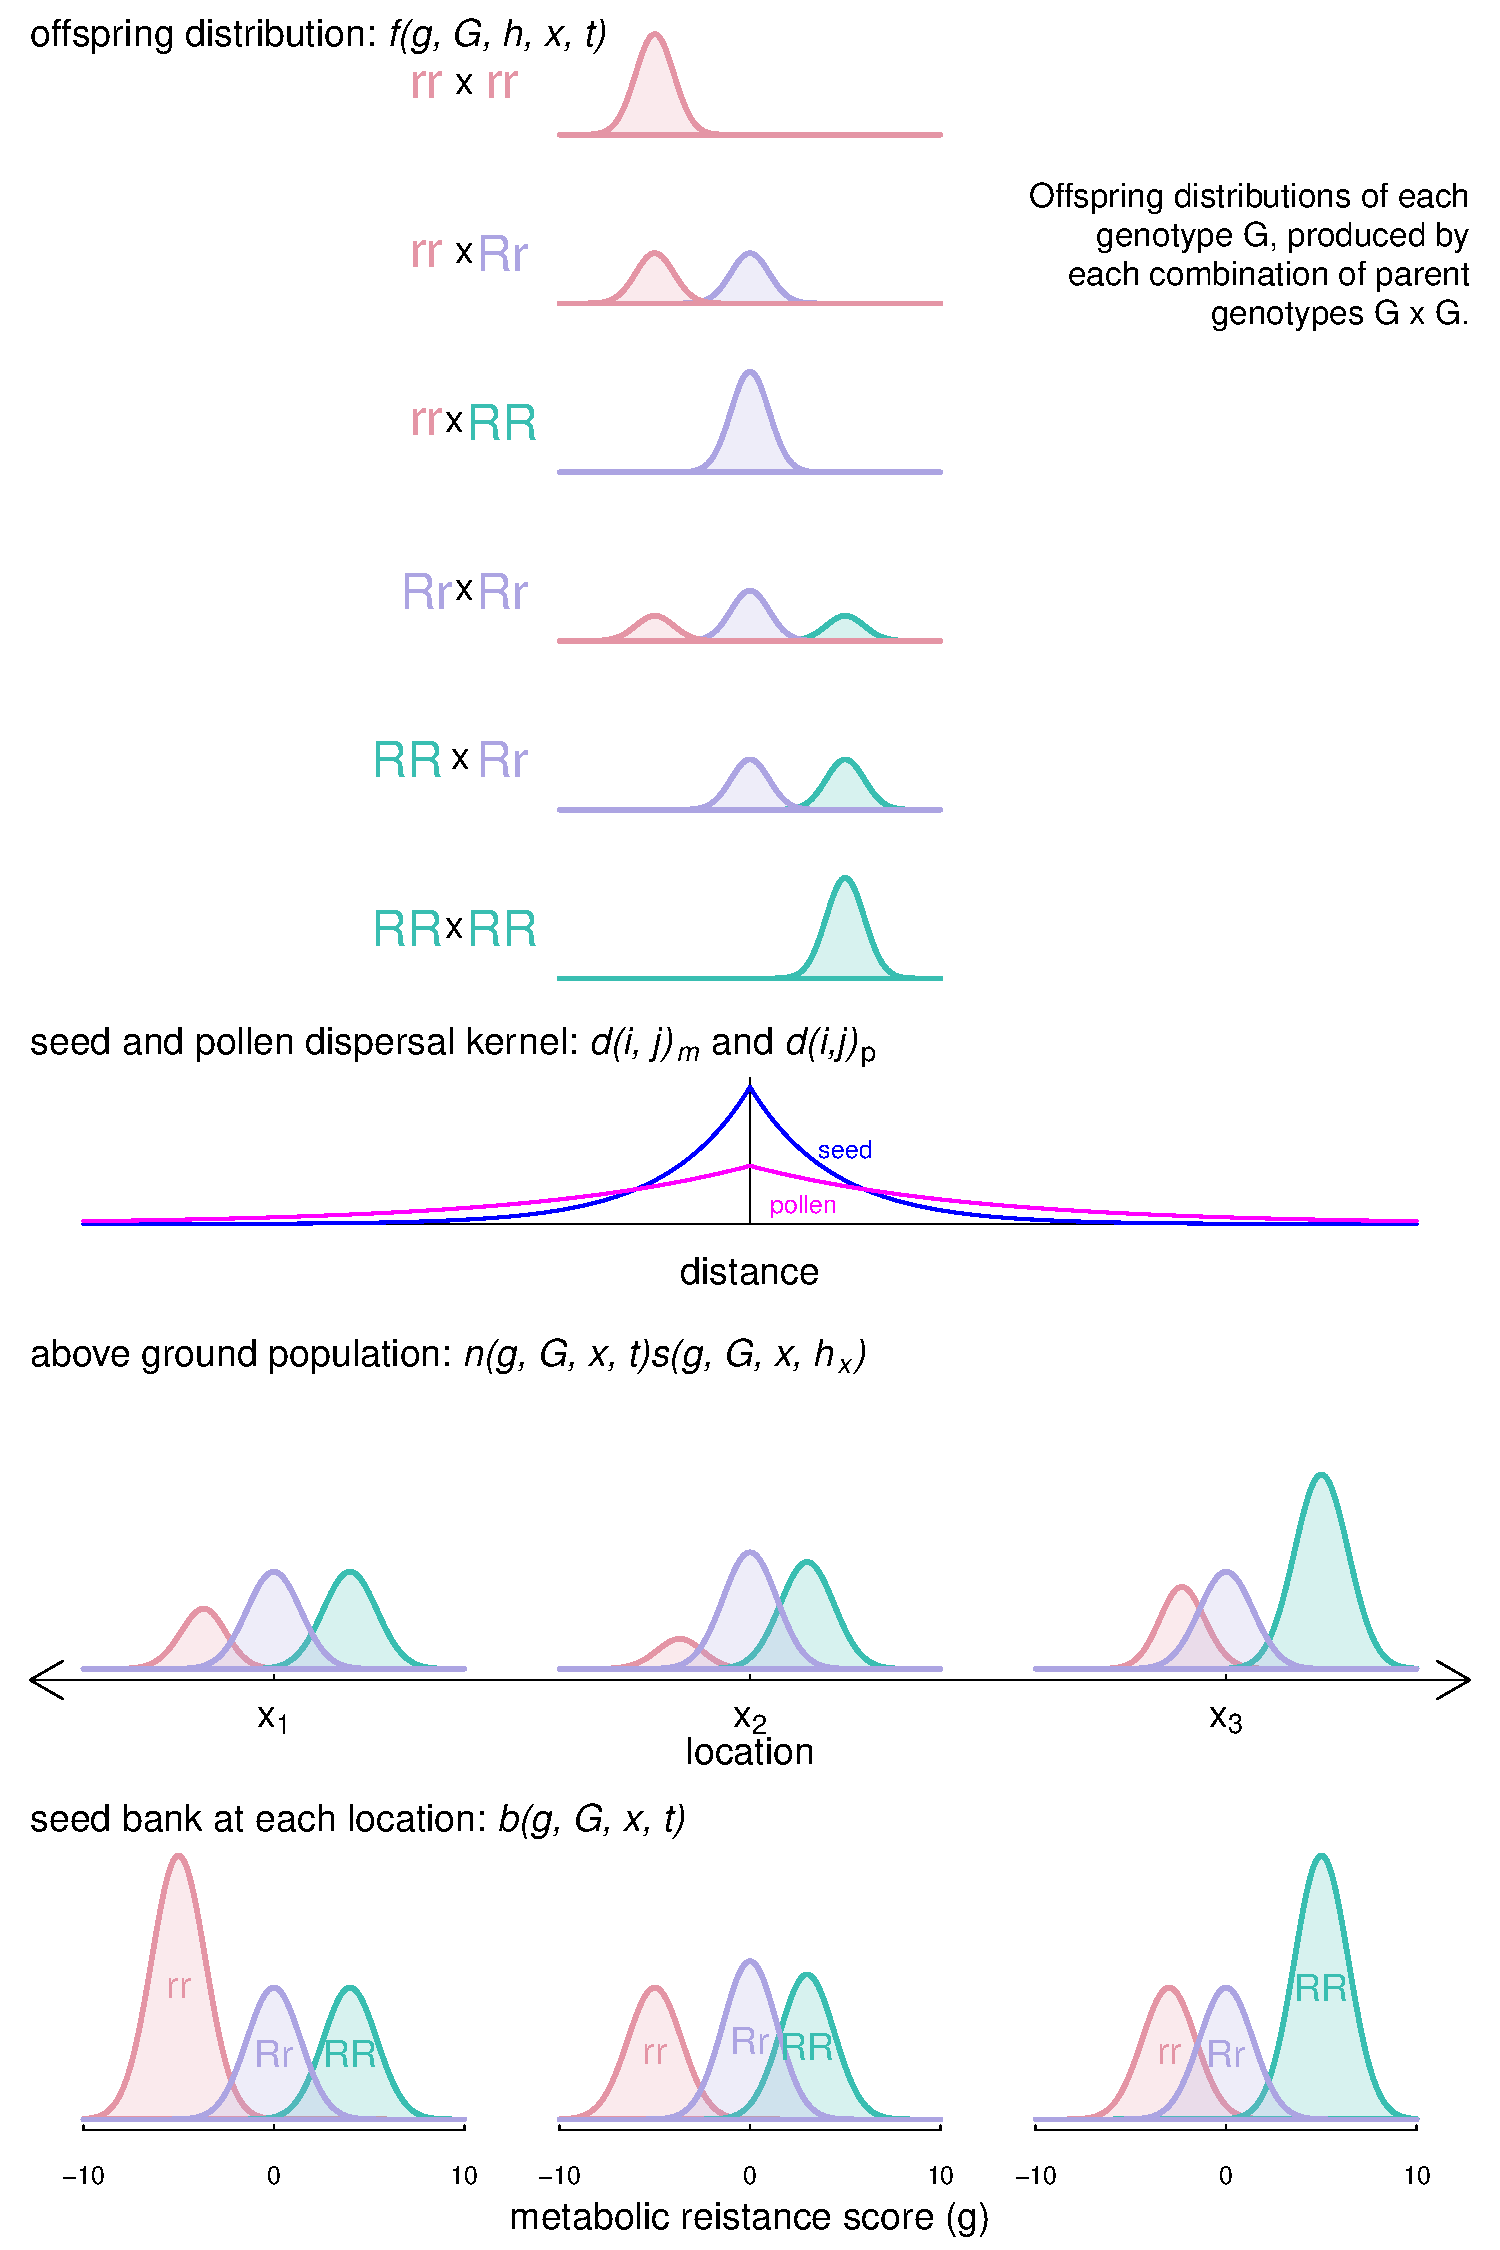
\includegraphics[height=200mm]{/home/shauncoutts/Dropbox/projects/MHR_blackgrass/BG_population_model/writting/spatial_model_fig/BG_pop_spatial_mod_schematic.pdf}
\caption{Schematic of the spatial population model. At each location $x_i$ seeds in the the seed bank have one of three target site resistance genotypes $G \in \{RR, Rr, rr\}$ and are distributed over metabolic resistance score $g$. The emergence and survival functions, $n(g, G, x, t)s(g, G, x, h_x)$ are applied to the seed bank distributions to get the above ground parent distributions. Those above ground distributions of survivors are the parent distributions that mix across genotypes and locations (via the pollen dispersal kernel) to create the offspring distributions. Seeds are then dispersed between locations using the seed dispersal kernel.}
\end{figure}

\end{document}